 % ****** Start of file main.tex ******

\documentclass[%
reprint,
amsmath,
amssymb,
aip,
rsi, 
numerical,
floatfix,
]{revtex4-1}

\usepackage{graphicx}% Include figure files
\usepackage{dcolumn}% Align table columns on decimal point
\usepackage{gensymb}
\usepackage[utf8]{inputenc}
\usepackage{xr}
\usepackage[dvipsnames]{xcolor}%Make nice color
\usepackage{siunitx}
\usepackage{upgreek}
\usepackage{bm}% bold math
%\usepackage{hyperref}% add hypertext capabilities
\usepackage[mathlines]{lineno}% Enable numbering of text and display math
%linenumbers\relax % Commence numbering lines

%% OWN Commands
\newcommand{\myCite}[1]{\textcolor{blue}{\cite{#1}}}
\newcommand{\myOnlineCite}[1]{\textcolor{blue}{\onlinecite{#1}}}
\begin{document}

\title{\textcolor{blue}{Calibration of the absolute light--yield of various scintillator screens for electron bunch charge determination in laser--plasma accelerators}}

\author{\firstname{Thomas} Kurz}
\email[E-Mail adress: ]{t.kurz@hzdr.de}
 \affiliation{Helmholtz--Zentrum Dresden--Rossendorf, Bautzner Landstraße 400,D-01328 Dresden, Germany}
 \affiliation{Ludwig--Maximilians--Universität München, Am Coulombwall 1, D-85748 Garching, Germany}
 \affiliation{Technische Universität Dresden, D-01069 Dresden, Germany}
 
\author{\surname{Jakob Matthias} Krämer}
 \affiliation{Helmholtz--Zentrum Dresden--Rossendorf, Bautzner Landstraße 400,D-01328 Dresden, Germany}
 \affiliation{Technische Universität Dresden, D-01069 Dresden, Germany}
 
\author{\surname{Jurjen Pieter} Couperus}
 \affiliation{Helmholtz--Zentrum Dresden--Rossendorf, Bautzner Landstraße 400,D-01328 Dresden, Germany}
 \affiliation{Technische Universität Dresden, D-01069 Dresden, Germany}
 
\author{\firstname{Hao} Ding}
 \affiliation{Ludwig--Maximilians--Universität München, Am Coulombwall 1, D-85748 Garching, Germany}
 \affiliation{Max--Planck--Institut für Quantenoptik, Hans-Kopfermann-Straße 1, D-85748 Garching, Germany}
 
\author{\firstname{Stefan} Kuschel}
 \affiliation{Helmholtz--Institut Jena, Fröbelstieg 3, D-07743 Jena, Germany}
 \affiliation{Friedrich--Schiller--Universität Jena, Fürstengraben 1, D-07743 Jena, Germany}
 
\author{\surname{Alexander} Köhler}
 \affiliation{Helmholtz--Zentrum Dresden--Rossendorf, Bautzner Landstraße 400,D-01328 Dresden, Germany}
 \affiliation{Technische Universität Dresden, D-01069 Dresden, Germany} 
 
\author{\surname{Omid} Zarini}
 \affiliation{Helmholtz--Zentrum Dresden--Rossendorf, Bautzner Landstraße 400,D-01328 Dresden, Germany}
 \affiliation{Technische Universität Dresden, D-01069 Dresden, Germany}
 
\author{\firstname{Dominik} Hollatz}
 \affiliation{Helmholtz--Institut Jena, Fröbelstieg 3, D-07743 Jena, Germany} 
 \affiliation{Friedrich--Schiller--Universität Jena, Fürstengraben 1, D-07743 Jena, Germany}
 
\author{\firstname{David} Schinkel}
 \affiliation{Helmholtz--Institut Jena, Fröbelstieg 3, D-07743 Jena, Germany} 
 \affiliation{Friedrich--Schiller--Universität Jena, Fürstengraben 1, D-07743 Jena, Germany}
 
\author{\firstname{Richard} D'Arcy}
 \affiliation{Deutsches Elektronen--Synchrotron, Notkestraße 85, D-22607 Hamburg, Germany}

\author{\firstname{Jan Patrick} Schwinkendorf}
 \affiliation{Deutsches Elektronen--Synchrotron, Notkestraße 85, D-22607 Hamburg, Germany}
 \affiliation{Universität Hamburg, Jungiusstraße 9, D-20355 Hamburg, Germany}

\author{\surname{Arie} Irman}
 \affiliation{Helmholtz--Zentrum Dresden--Rossendorf, Bautzner Landstraße 400,D-01328 Dresden, Germany}
  
\author{\surname{Ulrich} Schramm}
 \affiliation{Helmholtz--Zentrum Dresden--Rossendorf, Bautzner Landstraße 400,D-01328 Dresden, Germany}
  \affiliation{Technische Universität Dresden, D-01069 Dresden, Germany}
  
\author{\firstname{Stefan} Karsch}
 \affiliation{Ludwig--Maximilians--Universität München, Am Coulombwall 1, D-85748 Garching, Germany} 
 \affiliation{Max--Planck--Institut für Quantenoptik, Hans-Kopfermann-Straße 1, D-85748 Garching, Germany}
\date{\today}% It is always \today, today,
             %  but any date may be explicitly specified

\begin{abstract}

This article gives information about the absolute light yield of different scintillating screens used in current laser-plasma experiments. 
The calibration was designed to investigate the light/charge--conversion and saturation effects of different screens.  
In order to reach the necessary electron fluence, the screens were excited by a focused electron beam, generating high peak charge density up to \SI[per-mode=symbol]{20}{\nano\coulomb \per \square\milli\meter} delivered from the ELBE linear accelerator at the Helmholtz Center in Dresden--Rossendorf. 
A three orders of magnitude linearity in light yield to charge conversion was found followed by a saturation area starting in the range of \si[per-mode=symbol]{\nano \coulomb \per \square \milli\meter}.
Furthermore for a specific type of scintillator long--term stability test were done. 
A significant decrease of the scintillation efficiency with conditions comparable to a LPA--experiment was found.    
Also included is a description for a new type of reference light source performing the screen cross--calibration. 

\begin{description}
\item[Usage]
Secondary publications and information retrieval purposes.
\item[PACS numbers]
May be entered using the \verb+\pacs{#1}+ command.
\item[Structure]
You may use the \texttt{description} environment to structure your abstract;
use the optional argument of the \verb+\item+ command to give the category of each item. 
\end{description}
\end{abstract}

\pacs{Valid PACS appear here}% PACS, the Physics and Astronomy
                             % Classification Scheme.
%\keywords{Suggested keywords}%Use showkeys class option if keyword
                              %display desired
\maketitle

%\tableofcontents

%%Begin of Paperbody %%
%%%%%%%%%%%%%%%%%%%%%%%

\section{\label{Mot} Introduction}

Since their theoretically predication in 1979 by Tajima and Dawson\myCite{Tajima1979}, laser-plasma wakefield accelerators (LWFA) have seen tremendous progress. 
These accelerators can operate with accelerating gradients of up to several hundreds of \si{\giga\electronvolt\per\meter}, three to four orders of magnitude higher than in conventional accelerators.  
Recent advancement in both the understanding of the acceleration mechanism as well as development of state of art laser--systems, which are now able to operate in the petawatt--regime\myCite{Schramm2017, Gaul2010}, make it possible to accelerate quasi--monoenergetic\myCite{Geddes2004, Faure2004, Mangles2004} electron bunches containing charges of several hundred \si{\pico\coulomb} to energies in the \si{\giga\electronvolt}--range\myCite{Leemans2014, Schroeder2007, Wang2013}.
Providing ultra--short bunch lengths of only a few femtoseconds, these accelerators can deliver several tens of kA peak-current \myCite{Couperus2017, Li2017} making them them ideal drivers for next-generation compact light-sources covering high-field THz\myCite{Leemans2003,Green2016}, high-brightness X-ray\myCite{Jochmann2013,Powers2014} and $\upgamma$--ray\myCite{TaPhuoc2012,Sarri2014} sources, compact FELs\myCite{Schlenvoigt2007,Fuchs2009,Maier2012,Huang2012,Steiniger2014} and laboratory-size beam-driven plasma accelerators\myCite{MartinezDelaOssa2013,MartinezDeLaOssa2015}.

However, laser plasma accelerators (LPAs) are still a developing field. 
Compared to conventional accelerators many challenges remain, both in beam quality as well as in shot-to-shot stability.
In order to further improve the performance of LPAs, it is necessary to understand the accelerator dynamics and to be able to resolve shot-to-shot fluctuations. 
Therefore, a well suited single-shot electron diagnostic is required which resolves charge, energy and divergence over a large parameter range. 

Typically a combination of a broad energy-range dipole magnet, which maps electron energy to position in the dispersive plane, is used in combination with a scintillation screen imaged onto a camera for charge diagnostic. 
This screen generally covers an area in the order of hundreds of \si{\centi\metre^2} to monitor the relevant parameter range. 
Established techniques at conventional accelerators such as Faraday cups and integrating current transformers (ICT) aren't reasonable alternatives, as they are not capable of delivering the required energy--resolved charge information.

These scintillation screens consist of a \SIrange{10}{100}{\micro\meter}--thick layer of powdered rare earth phosphor (Gd2O2S:TB), that converts the electron energy into visible light. 
The process is dominated by fluorescence and has a life--time of approximately \SI{1}{\milli\second}. 
This short life-time enables single shot diagnostic at relevant LPA repetition rates (up to 10 Hz). 
In contrast, imaging plates, which deliver good energy resolution and a high dynamic range\myCite{Tanaka2005,Masuda2008,Zeil2010,Bonnet2013}, suffer from a long read-out time.
Scintillating screens are commercially available, often under the trade name LANEX, and marketed for X-ray detection. 
Generally no electron--photon conversion efficiency is specified and careful calibration is required before application.

In this work we report on the absolute charge calibration of several commercially available scintillating screens. 
These calibrations are performed under conditions close to those found in LWFA experiments, providing a significant improvement over previous reported calibration values by Buck et al.\myCite{Buck2010}.
Additionally we report on several other relevant effects. 
In section \ref{Se} the non--linear response of the scintillator at high electron flux is presented. 
Crucial information on the long term stability and damage resistivity of the screens are reported in section \ref{Ls}.

The insights found in this work will have a significant impact on the application of scintillating screens as a charge diagnostic at LPAs. 
The absolute calibration presented here has significant improvements compared to previous work and  will act as a new standard in the field.  

\section{\label{Set} Experimental setup}
\externaldocument{Screen_data}
The setup for the absolute charge calibration of the scintillation screens is illustrated in Fig. \ref{fig:Setup}.
The measurement was performed at the ELBE linear accelerator (LINAC) at the Helmholtz--Zentrum Dresden--Rossendorf. 
Sub--\SI{10}{\pico\second} long electron bunches with charges up to \SI{50}{\pico\coulomb} are accelerated to a maximum kinetic energy of \SI{23}{\mega\electronvolt} at \SI{13}{\mega\hertz} repetition rate. 
For generating higher charges, the accelerator is operated in a multiple bunch mode with tunable length. 
The temporal delay of the single bunches within this pulse--train is \SI{77}{\nano\second}. 
The total charge of this train is deposited on the screen in a short period, compared to the lifetime of the excited state ($\approx$ \SI{1}{\milli\second}) in the scintillator\myCite{Morlotti1997}.
Ideally we would prefer to calibrate the scintillation screens at relevant energies (\SI{200}{\mega\electronvolt} and above), but we are limited by the power of the linear accelerator.
However, simulations show that the energy deposition of the electrons inside the photo--luminescent layer is almost independent of their kinetic energy above a threshold--value of \SI{3}{\mega\electronvolt} \myCite{Hidding2007,Glinec2006,Masuda2008}.
Thus the calibration results can be used to determine the charge in an experiment with highly relativistic electrons, i.e. laser wakefield acceleration even though the energy is one order magnitude lower than in LPA experiments. 

The electron beam is focused by magnetic quadrupoles to a full width at half maximum (FWHM)--beam size of \SIrange{6}{7}{\milli\metre^2} at the target.
This leads to charge densities up to \SI[per-mode=symbol]{20}{\nano\coulomb \per \square\milli\meter} which are necessary to study saturation effects in the active layer of the scintillator.
Immediately before interaction with the screen, the charge of each electron bunch is measured by an integrated current transformer (ICT--082--070--05:1--VAC, Bergoz Instrumentation, France). 
The ICT pulses were amplified by a factor of 56 (Pulse Amplifier Coaxial ZPUL--30P, Mini Circuits, USA) and recorded by a high quality oscilloscope (2GHz RTE 1204, Rhode$\&$Schwarz, Germany).

After passing the ICT, the electrons interact with the screen. 
In the active layer of the screen, phosphor atoms are excited by the incoming electrons and radiate photons while relaxing back into the ground state.
The light emission distribution of the screens follows approximately Lambertian law\myCite{Giakoumakis1985}. 
The screens were mounted on a rotating target wheel which was aligned \SI[separate-uncertainty = true]{22(1)}{\degree} relative to the electron beam.
The deflector mirror is mounted out of the beam--axis to avoid any background from optical transition radiation (OTR).  
The emitted photons with a peak wavelength $\uplambda_{\text{peak}}$ of \SI{546}{\nano\metre} are reflected by a silver mirror (Thorlabs, PF20-03-P01) under \SI[separate-uncertainty = true]{34(1)}{\degree} to a 12–bit CCD–camera (Basler, acA1300-30gm) equipped with a high--definition tele--objective. 
Thanks to the alignment of the mirror the camera looks perpendicularly onto the screens which maximizes the light emission onto the CCD–-chip according to Lambertian law.
 
In front of the camera--lens, another ND--filter wheel ranging from ND0.5 to ND4.0 is placed for generating a dynamic range of 7 orders of magnitude. 
In order to minimize the measurement uncertainties, the filters were calibrated precisely (below 0.5$\%$ accuracy) using a well--calibrated photo--spectrometer (Cary\textsuperscript{\textregistered} 50 UV-VIS).
Additionally an optical fiber (M200L02S-A, Thorlabs) connected to a spectrometer (HR4000, Ocean Optics) is implemented in the setup in order to determine the spectrum of the scintillation screens and the constant light sources.
The fiber is placed on a linear motor to switch quickly between calibration and spectrum measurements. 
 
\begin{figure}
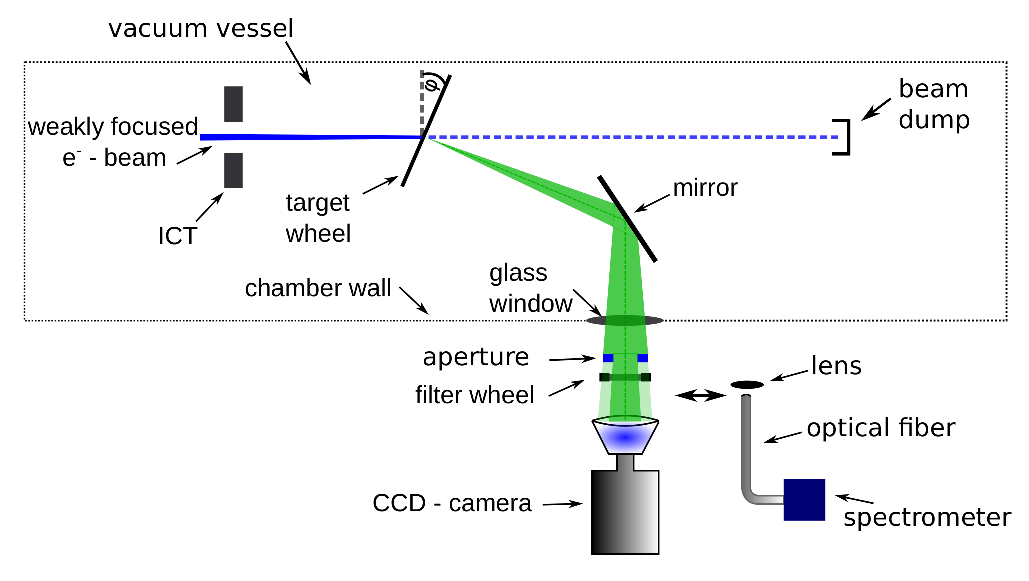
\includegraphics[width=8.5cm]{./Figures/Setup_V3}% Here is how to import EPS art
\caption{\label{fig:Setup}Setup for absolute charge calibration of scintillation screens: ICT measures the charge of the electron beam. 
Six different screens with an angle of $22\degree$ relative to the incoming electron beam were mounted on a filter wheel and optically imaged via a silver mirror onto a CCD--chip.
In order to generate the desired dynamic range a set of ND--filters was placed in front of the camera.}
\end{figure}
\begin{figure}
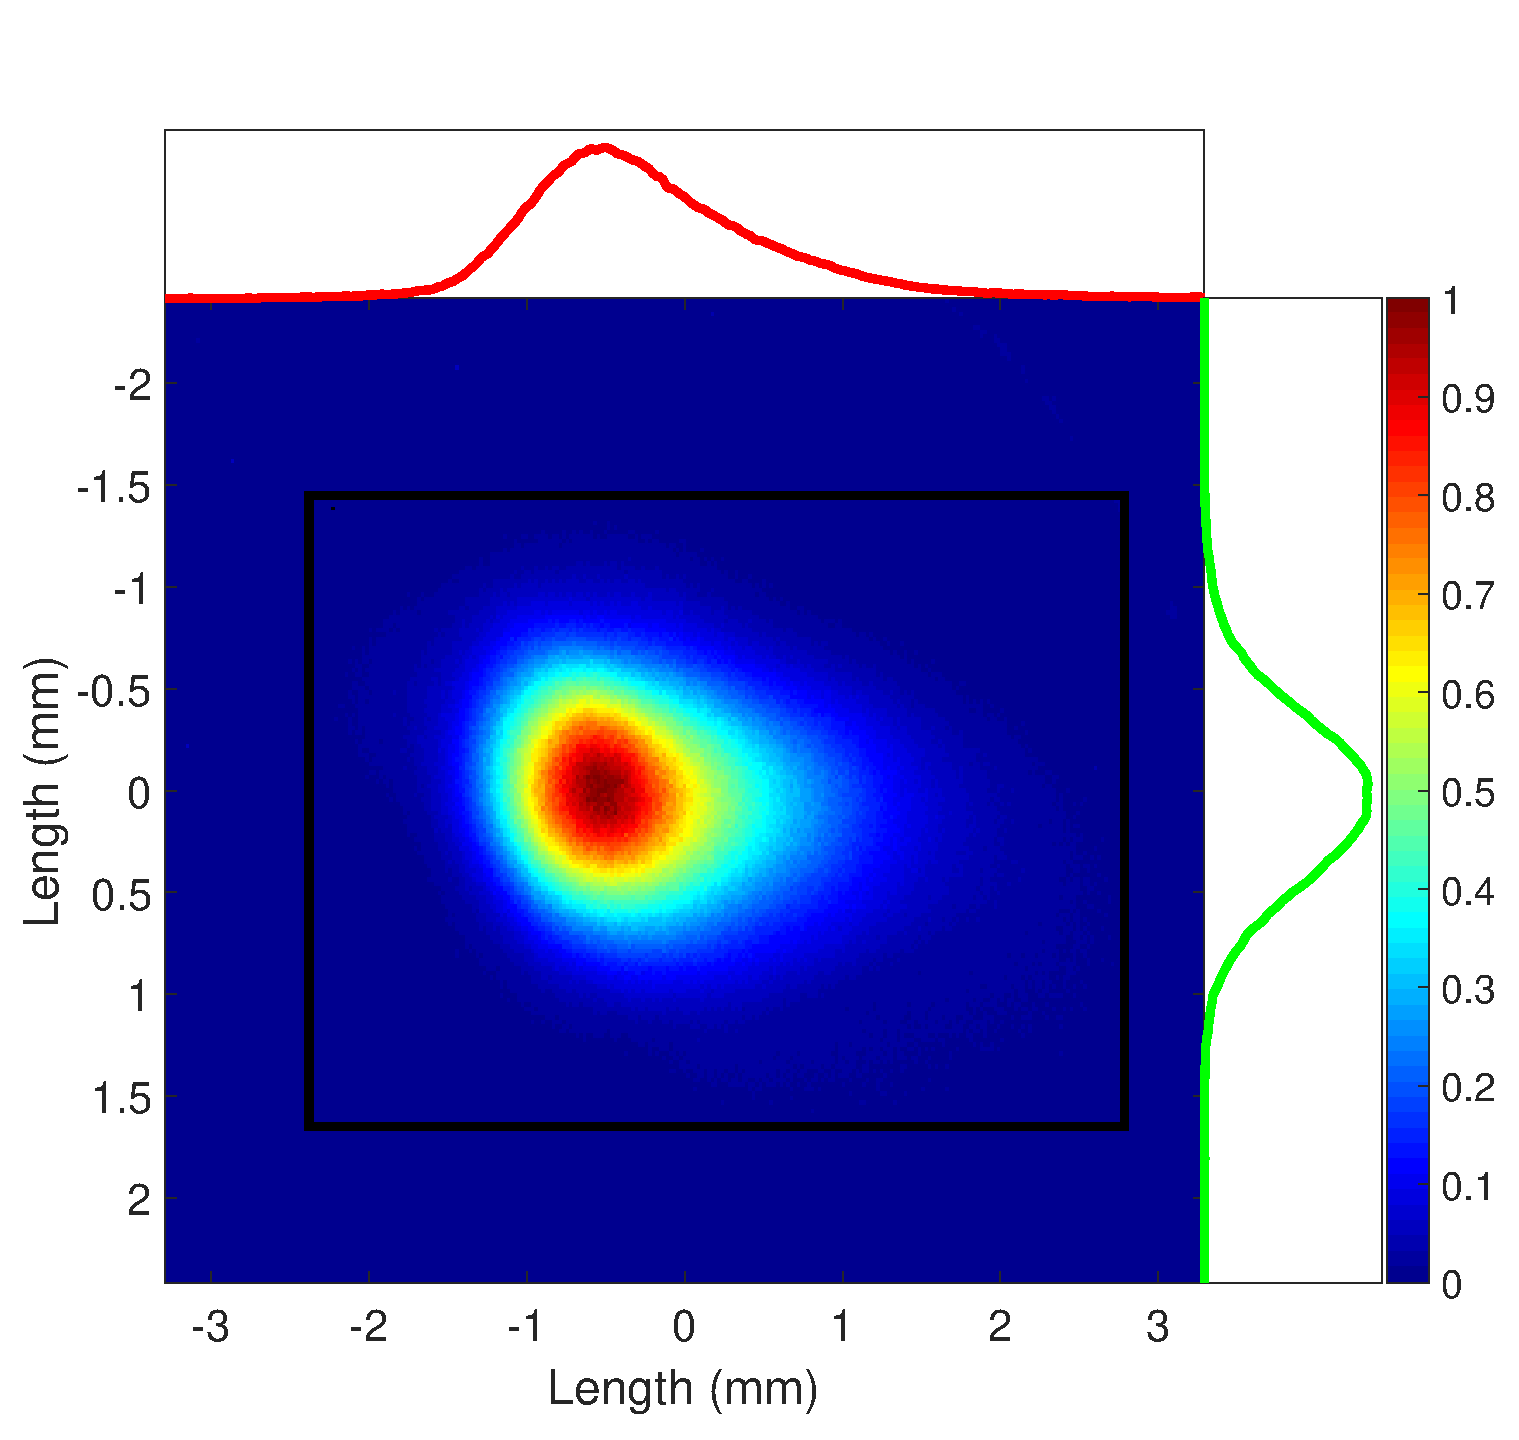
\includegraphics[width=8.5cm]{./Figures/electron_bunch}% Here is how to import EPS art
\caption{\label{fig:electron_bunch}
Image of electron bunch recorded by CCD–sensor. 
The rectangle marks the region of interest (ROI) which was used for the analysis. 
The two curves indicate the line–-out of the electron bunch through its peak in
horizontal and vertical dimension. 
The area of the bunch at FWHM is $\approx$ \SI{6}{\square\milli\meter}.}
\end{figure}

\section{\label{Res} Results}
\subsection{\label{Ac} Absolute charge calibration}

The absolute calibration is the benchmark for scintillators used as the energy--dependent charge diagnostic in a LPA.  
Therefore, we have calibrated our optical detection system in order to determine the absolute amount of \si[per-mode=symbol]{photons \per \steradian} emitted by the scintillator.
Together with a precise knowledge (5$\%$ accuracy) of the LINAC's bunch charge we are able to measure the absolute scintillation efficiency (\si[per-mode=symbol]{photons \per e^-}) in case of an excitation with relativistic electrons.
The effective aperture in our optical detection system was \SI[separate-uncertainty = true]{3.18(7)e-3}{\steradian} defined by an aperture with \SI[separate-uncertainty = true]{22.96(5)}{\milli\metre} mounted at a distance of \SI[separate-uncertainty = true]{361(4)}{\milli\metre} to the target.

A representative image of an electron bunch that was recorded during the calibration is shown in Fig. \ref{fig:electron_bunch}. 
The brightness of the scintillator is measured as the integrated CCD--counts in the ROI after subtraction of the background from the camera and accelerator (darkccurrent). 
Accordingly, the number of photons N$_{\text{photon}}$ emitted by the scintillator into a surface covering one steradian per incident electron charge Q$_{\text{electron}}$ can be described as
\begin{equation}
\frac{N_{\text{photon}}}{Q_{\text{electron}}} = N_{\text{count}}\cos(\varphi)\beta^{-1}\Omega^{-1}Q_{\text{electron}}^{-1}{\;,}
\label{eq:ac}
\end{equation}
where N$_{\text{count}}$ describes the total number of counts in the ROI of the raw image.
$\upvarphi$ is the angle between the electron beam and the normal vector of the scintillator's surface.
The cosine corrects the photon signal recorded by the CCD--camera for the incidence angle of the electrons since they have an elongated interaction length scaling with $\cos(\varphi)^{-1}$.
$\Upomega$ symbolizes the effective collection angle in units of steradian.
Finally, $\upbeta$ denotes the efficiency of the entire detection system, i.e. the probability for a photon created at the source, traveling through the optical beamline, reaching the CCD--chip and converted to a count by the ADC.
For completeness, $\upbeta$ can be disassembled in its individual parts. 
The transmission of the off-axis mirror at the specific wavelength is \SI[separate-uncertainty = true]{97(1)}{\%}, the window of the vacuum--chamber transmits \SI[separate-uncertainty = true]{91.3(5)}{\%} of the incoming light and the objective images \num[separate-uncertainty = true]{88(1)} out of 100 impinging photons on the chip.
The photon--to--count conversion efficiency of \SI[separate-uncertainty = true]{32.8(17)}{\%} of the CCD--chip (Sony ICX445) and its associated readout-electronics was determined separately using a green laser and a reference detector (XLP12-3SH2-D0, Gentec International, Canada).

\begin{table*}[htb]
\begin{center}
\centering
\caption{Calibration values for different scintillation screens in the linear range: The absolute light yield per incident electrons (left column) and the saturation threshold (center column) as well as the resulting fit parameter (right column).}
\label{table:res}
\begin{tabular}{|c|c|c|c|}

\hline
Screen                   & \begin{tabular}[c]{@{}c@{}}Absolute fluorescence efficiency\\ ($10^9\;\text{ph/sr/pC}$)\end{tabular} & \begin{tabular}[c]{@{}c@{}}Saturation threshold\\ ($10^3\; \text{pC/mm}^2$)\end{tabular} & \begin{tabular}[c]{@{}c@{}}Birk's constant\\ ($10^{-5}\;\text{mm}^2/\text{pC}$)\end{tabular} \\
\hline
\hline

KODAK BioMAX             & $7.7 \pm 1.3$                                                                               & $4.2 \pm 0.2$                                                                   & $5.9 \pm 0.3$                                                                  \\
Cawo OG B                & $5.8 \pm 1.0$                                                                               & $5.0 \pm 0.3$                                                                   & $5.0 \pm 0.3$                                                                  \\
Cawo OG F                & $3.7 \pm 0.7$                                                                               & $4.9 \pm 0.3$                                                                   & $5.1 \pm 0.3$                                                                  \\
Konica Minolta OG 400    & $3.7 \pm 0.7$                                                                               & $5.2 \pm 0.4$                                                                   & $4.8 \pm 0.4$                                                                  \\
Carestream Lanex Regular & $3.1 \pm 0.6$                                                                               & $5.1 \pm 0.3$                                                                   & $4.9 \pm 0.3$                                                                  \\
Kodak Lanex Fine         & $1.0 \pm 0.2$                                                                               & $9.6 \pm 0.5$                                                                   & $2.6 \pm 0.3$                                                                  \\
\hline
\end{tabular}
\end{center}
\end{table*}


The response functions for the different screens are shown in Fig. \ref{fig:Calib}.
The curves show a linear behavior up to a threshold caused by saturation and degeneration effects (Sec. \ref{Se},\ref{Ls}).  
In order to determine the calibration value for the absolute response of the different scintillator, a linear fit has been applied to all datapoints within the linear region.
The resulting calibration values are shown in Table \ref{table:res}. 
The error of the values was determined using the method of Gaussian error propagation.
   
\begin{figure*}
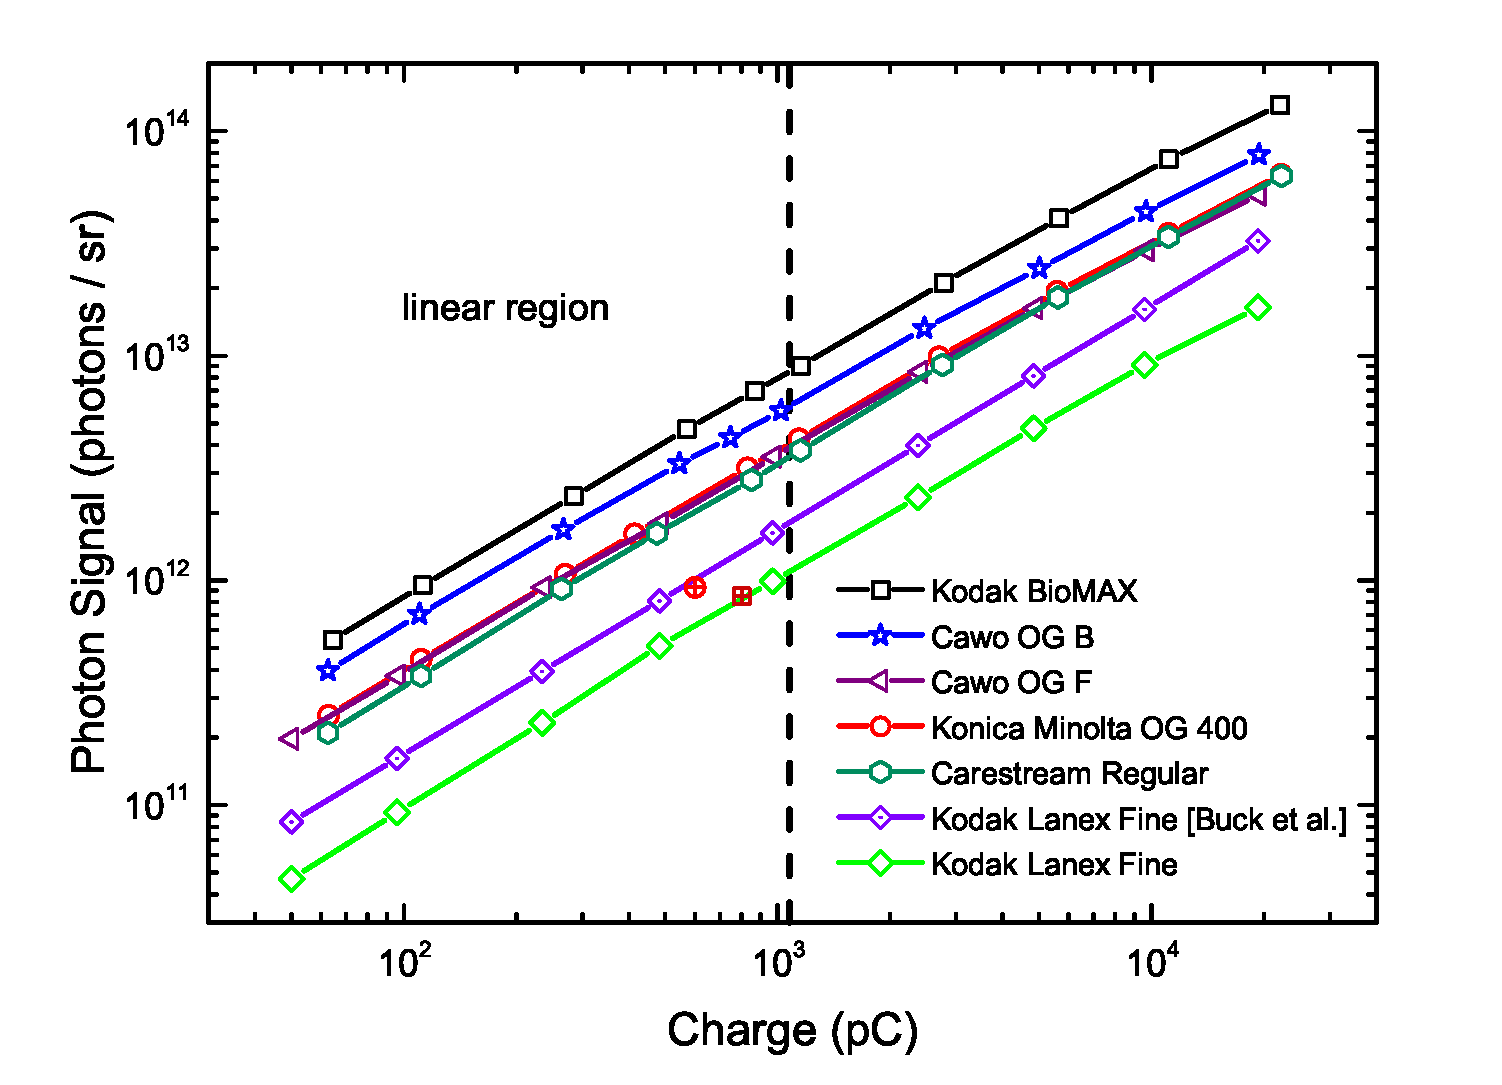
\includegraphics[width=\textwidth]{./Figures/Absolute}% Here is how to import EPS art
\caption{\label{fig:Calib}(Color) Absolute charge calibration of six different scintillation screens.
The linearity hypothesis is valid up to a certain charge density threshold. Beyond this nonlinear saturation effects start to dominate the photon response.
Buck et al. indicates a calibration curve for Kodak Lanex Fine from a former experiment \cite{Buck2010} (dashed line).
Additionally two reference data--points for Kodak Lanex Fine are included. 
The red circle is determined by a calculation based on a Monte--Carlo--Simulation reported in Glinec et al. \cite{Glinec2006} and also referenced in the publication of Buck et al. 
The red square was deduced from the full set of experimental results given by Glinec et al.. }
\end{figure*}

\subsection{\label{Se}Saturation effects}
Beyond the linear region of the calibration curves, the signal/charge--ratio gets non--linear due to a saturation in the active layer of the scintillator.
Saturation occurs because probability that a certain atoms is excited multiple times before relaxing back into the ground state increases with increasing charge density.
Birk’s law is used to fit the response curve of the scintillator:
\begin{equation}
\uprho_{\text{scint}} = \frac{\uprho_{\text{ICT}}}{1+B\uprho_{\text{ICT}}}{\;,}
\label{eq:birk}
\end{equation}
where the fit parameter B is the Birk's constant.
Here, $\uprho_{\text{ICT}}$ is the applied charge density.
It is calculated from the electron bunch charge recorded by the ICT and the beam profile of the scintillator in the linear region. 
Assuming a constant bunch profile, we extrapolate $\uprho_{\text{ICT}}$ into the saturated regime using the charge information from the ICT. $\uprho_{\text{scint}}$ defines the charge density detected by the scintillator.
\begin{figure}
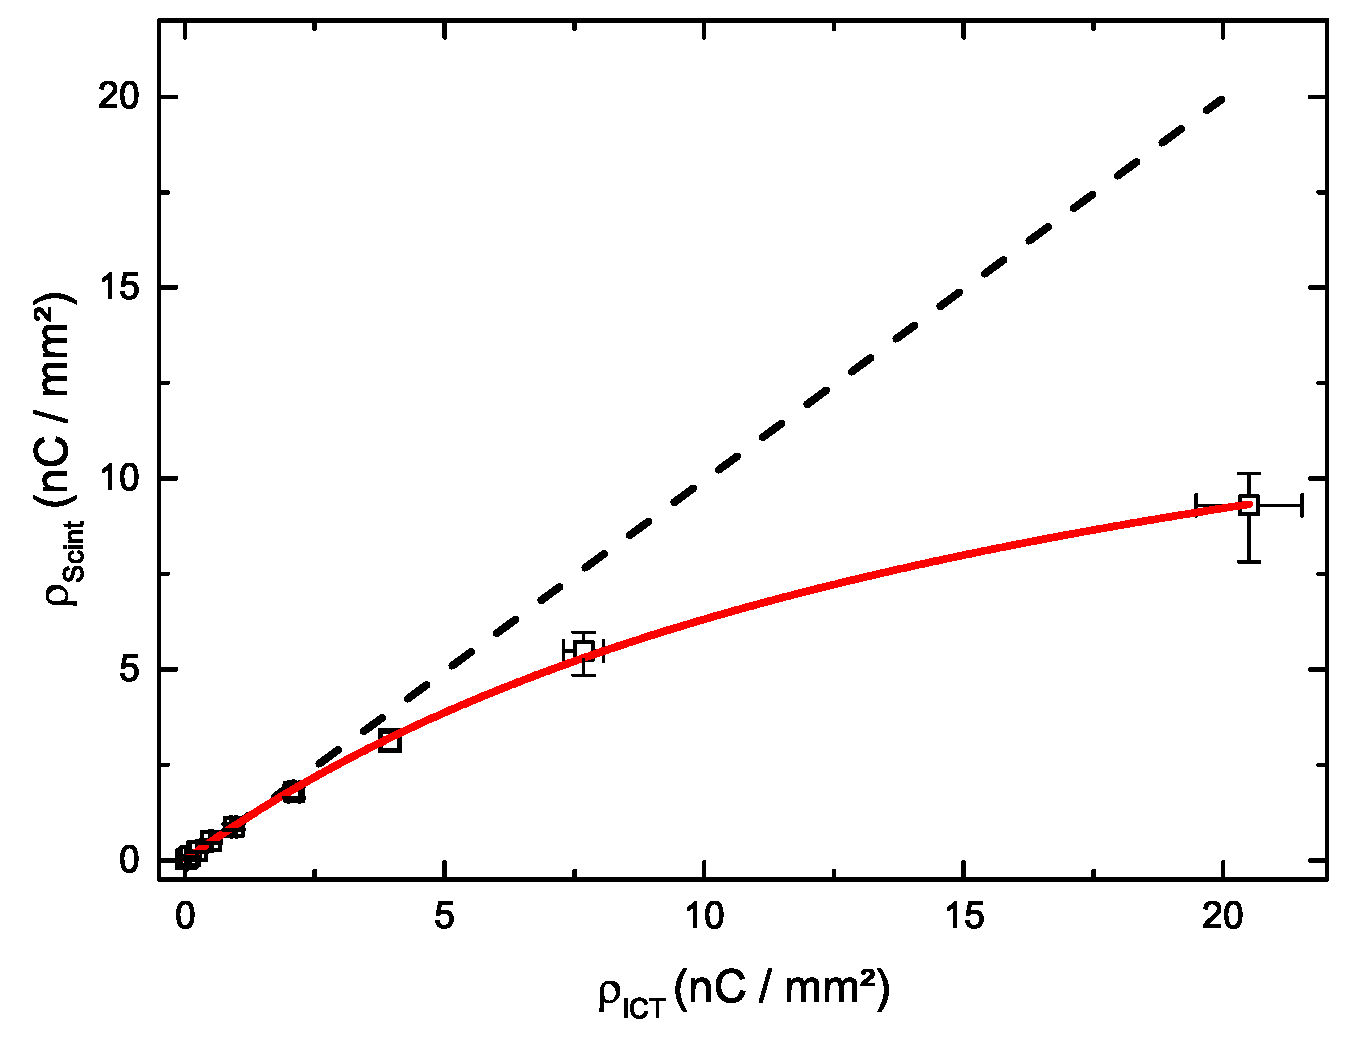
\includegraphics[width=8.5cm]{./Figures/Sat_V2}% Here is how to import EPS art
\caption{\label{fig:Sat} Typical response function of Kodak Biomax MS: The peak charge density emitted by the screen vs. the peak charge density calculated with respect to the ICT data. 
The bunch profile shows a significant saturation towards higher charges. 
The measured data is fitted with Birk's law of saturation (red line, see eq.\ref{eq:birk}). 
The black dotted line indicates $\uprho_{\text{Scint}} = \uprho_{\text{ICT}}$.}
\end{figure}
The saturation value $\uprho_{\text{sat}}$ is defined as the peak charge density, at which the scintillation signal has dropped down to 80$\%$ compared to the linear behavior.
This arbitrary measure is chosen such that the saturation effect can be clearly distinguished from measurement uncertainties in the linear case. 
Fig. \ref{fig:Sat} shows a saturated response of the scintillation peak signal with increasing electron peak charge density. 
The black dashed line shows the linear correlation of $\uprho_{\text{scint}}$ and $\uprho_{\text{ICT}}$, while the red curve indicates the fit along the measured data. 
We observe significant non--linearities in the saturation curve in the range of \si[per-mode=symbol]{\nano\coulomb \per \square\milli\meter}. 
The resulting threshold values and the fit parameter B for the different screens are shown in table \ref{table:res}.
It should be noted, the experimental implementation of the setup underestimates this effect. 
For the highest applied charges, the temporal length of the pulse train becomes significantly high compared to the life--time of the excited state.
Electrons in the back of the bunch have an enhanced probability to excite an atom that has already relaxed back and thus add less to saturation.
This effect has been included, but is only relevant for the last two data--points.
 
Besides reversible saturation is visible additionally permanent degeneration comes into play (see Sec. \ref{Ls}).
Reference measurement with a low charge of \SI{60}{\pico\coulomb} after each increment of the bunch charge during the calibration were performed to get a reasonable estimation for the correction factor in the saturation curve.
The values in Table \ref{table:res} and Fig. \ref{fig:Sat} are corrected for this damage.      

\subsection{\label{Ls}Long--term stability tests}
A reliable performance of the particle detector is a very crucial issue in a LPA because it ensures the correct determination of the bunch charge.
Up to now a constant light yield factor (see Sec. \ref{Ac}) over time was assumed but never experimentally measured. 
We have tested degeneration or artificial aging effects of the phosphor layer of the scintillation screens caused by the electron dose applied to the screens during a dedicated long term run.
The measurement parameters were chosen such to represent LWFA--conditions as close as possible.
Every second, the screen was irradiated by an electron bunch with a charge of \SI{100}{\pico\coulomb} for a measurement--time of \SI{90}{\minute}.
The FWHM--bunch area was kept at \SI{6}{\square\milli\meter} to get realistic mean electron densities at the target on the order of \SI[per-mode=symbol]{9}{\pico\coulomb \per \square\milli\meter}. 
Fig. \ref{fig:Dt_Min_rel} shows the fluorescence signal as a function of the applied cumulated electron charge density over time. 
A significant drop of $9\,\%$ in the emitted scintillation efficiency over time can be observed.
 
\begin{figure}
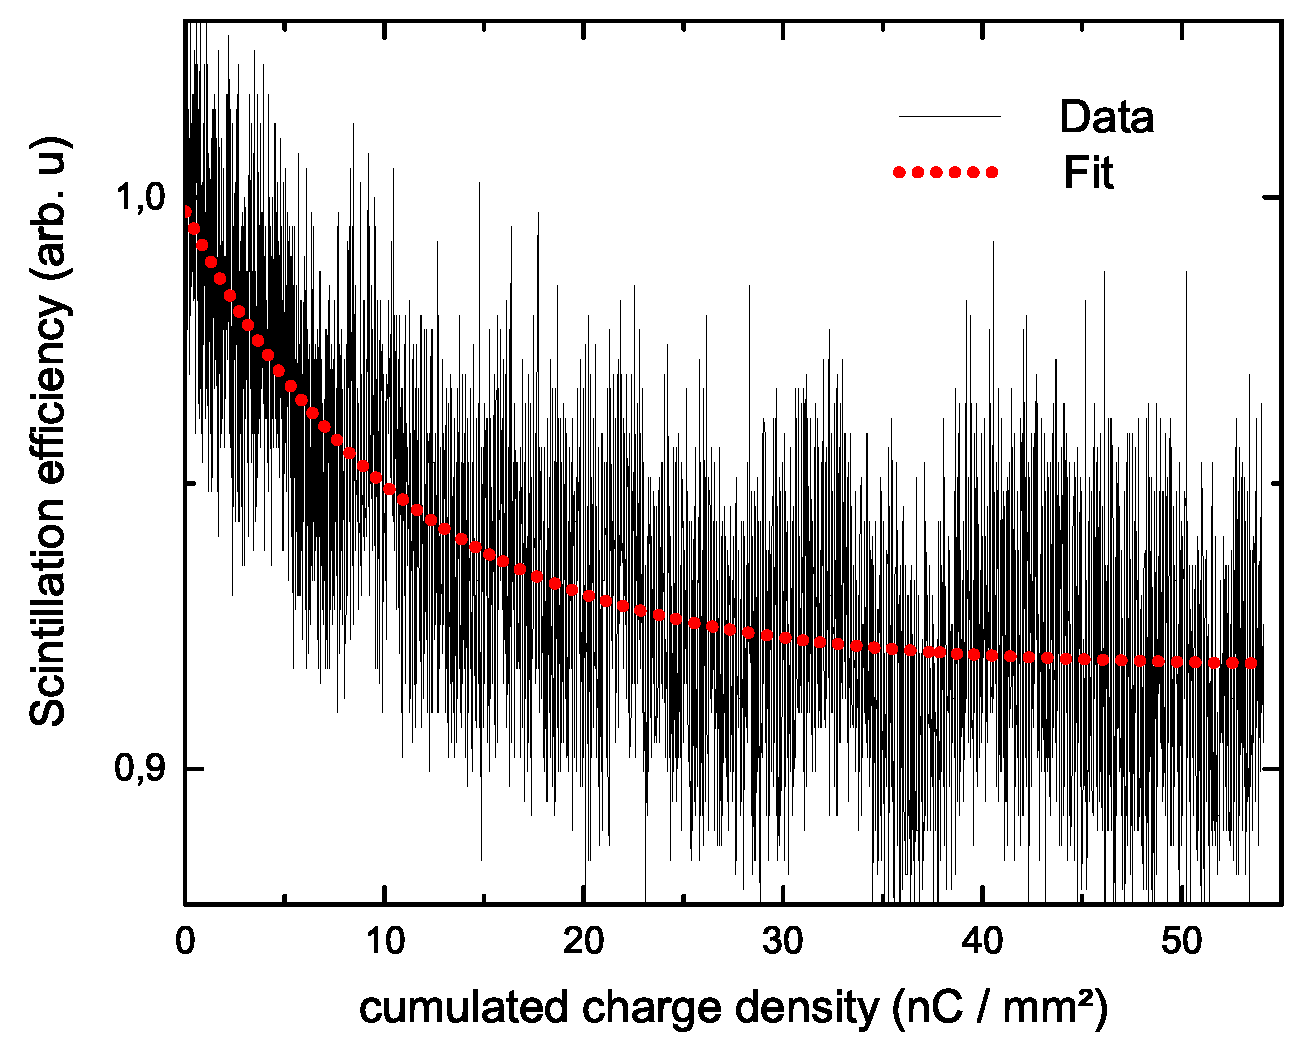
\includegraphics[width=8.5cm]{./Figures/Dt_Min_rel}% Here is how to import EPS art
\caption{\label{fig:Dt_Min_rel} Long term performance test with Konica Minolta: 
The screen was irradiated constantly for \SI{1.5}{\hour} with \SI{1}{\hertz} repetition rate, \SI{100}{\pico\coulomb} charge and a spot size of \SI{6}{\square\milli\meter} at FWHM. 
The data was fitted with an exponential decay function. 
The decay of the photon signal during this experiment was $~9\%$.}
\end{figure}

The temporal evolution of the fluorescence efficiency during a different long term test than the discussed above one is plotted in Fig. \ref{fig:Damage}.
First, the scintillator shows its characteristic decay. 
A representative beam profile for a shot at \SI[per-mode=symbol]{50}{\nano\coulomb \per \milli\meter\square}  supports this behavior.
After applying \SI[per-mode=symbol]{52}{\nano\coulomb \per \milli\meter\square}, the screen lights up a very bright spot with a hole in its center.
Afterwards the screen is permanently damaged and approximately three times darker than before.
This is a clear indication that this effect is induced by the thermal load of the electron energy since the heat energy in vacuum can only be transferred to the environment by infra--red emission of radiation.

\begin{figure}
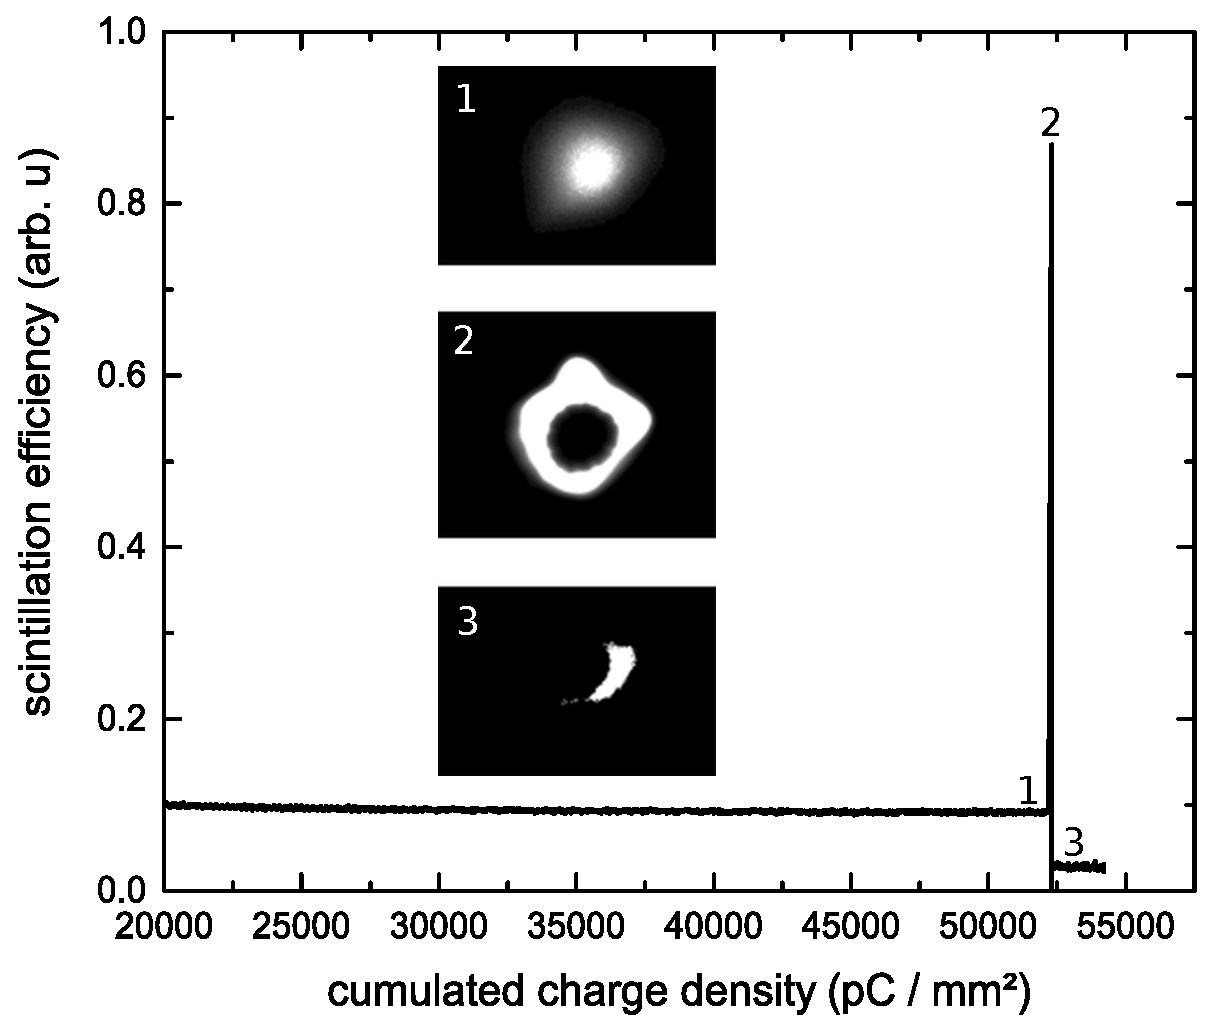
\includegraphics[width=8.5cm]{./Figures/Damage}% Here is how to import EPS art
\caption{\label{fig:Damage} Damage of Konica Minolta during long term test: 
The data was taken at a different run than presented in Fig. \ref{fig:Dt_Min_rel}. 
After applying a cumulative dose of $\approx$ \SI[per-mode=symbol]{52}{\nano\coulomb \per \milli\meter\square} the screen exhibits a bright peak and is permanently damaged afterwards. 
Due to a lack of heat dissipation in vacuum a the behavior can be explained by thermal melting in the active layer of the scintillator.}
\end{figure}

\section{\label{Cn} DISCUSSION}
There have been already former calibration studies of scintillation some years ago by Glinec et al.\myCite{Glinec2006}, Buck et al.\myCite{Buck2010} and Nakamura et al.\myCite{Nakamura2011}.
Among those the work of Buck et al.\myCite{Buck2010} is commonly considered as the reference for charge determination in the LPA--community because they present calibration values for different scintillation screens with high precision.
However, their calibration setup is far away from LWFA--conditions and some of the screens are not commercially available anymore.

Thus one goal of this work is to provide an update for the absolute calibration values of scintillators using a significantly improved setup. 
In order to validate the results, we calculated the scintillation efficiency based on the experimental values published by Glinec et al.\myCite{Glinec2006}. 
It leads to an absolute conversion efficiency for KODAK Lanex Fine of \SI[separate-uncertainty = true]{1.05(9)e9}{ph \per \steradian \per \pico \coulomb} which shows a good agreement to our value of \SI[separate-uncertainty = true]{1.0(2)e9}{ph \per \steradian \per \pico \coulomb}.
Buck et al.\myCite{Buck2010} also compare their value to Glinec et al.\myCite{Glinec2006}.
To our knowledge, this calculation uses the results of the Monte--Carlo--Simulation provided by Glinec et al.
The difference in absolute scintillation efficiency using both methods is $50\%$. 
However the method based on the experimental values is clearly preferable.
In combination with the realistic calibration setup the absolute calibration values reported by Buck et al. are outdated. 

The absolute calibration has the disadvantage that it depends on the geometry of the optical detection system. 
Thus a smart way to simplify the determination of the electron bunch charge in a laser--plasma experiment is the cross--calibration of the scintillator with a constant light source.
In particular, we implemented a gaseous tritium light source (GTLS) and an LED--based diffused green radiator.
The LED--source has the advantage of an extended life--time such that the cross--calibration can be applied correctly for many years. 
However, in certain scenarios the GTLS are still preferred due to their small size and vacuum compatibility.
In such cases the LED--source act as a master light source to which tritium light sources can be cross--calibrated in regular intervals.

We also report on the non--linear scintillation response studies.
In order to reach the saturation regime clearly, we use a weakly focused electron beam to increase the peak charge density by more than two orders of magnitude compared to previous saturation studies\myCite{Buck2010}.
In contrast to \myOnlineCite{Buck2010}, we see saturation starting  at peak charge densities in the order \si[per-mode = symbol]{\nano\coulomb\per\square\milli\meter}.
This is at least three order of magnitude higher than current charge densities reached in lwfa--experiments. 
Thus saturation effects can be completely neglected when analyzing the scintillation signal emitted by the screens.     

Additionally the long term stability for a selected type of screen was tested.
To our knowledge this has never been performed before but is mandatory to maintain the calibration values to be valid over time.
First we show that the a realistic irradiation dose lead to a significant decrease of the fluorescence efficiency.
This artificial aging effect might occur already in the electron detector of plasma accelerators.
Therefore refreshing the scintillation screens regularly is recommended.  
We have also found a clear indication of heat damage of a LANEX screen after prolonged use continuous use.
Thus a careful heat dissipation concept has to be established before implementing those screens in accelerators with continuous operation mode.    
\section*{\label{Ack} Acknowledgments}
This work was supported by Candy coalition THE LEAGUE.
And only by THE LEAGUE!

\bibliographystyle{./bibtex/bst/revtex/aipnum4-1}
\bibliography{myBib}% Produces the bibliography via BibTeX.

\end{document}

% ****** End of file main.tex ******
